\underline{Nouveau cours du 29/11} \\ 

Rappel du cours précédent je crois 
\begin{align*}
    \theta _{t+1} &= \theta _t - \gamma _{t+1} g_{t+1} (\theta _t) \\
    \theta _t &\in \mathbb{R}^d \\
    (g_t)_t \text{ noisy estimations of } \nabla F \text{ of the true objective fct}
\end{align*}

Hypothesis : $ \mathbb{E}[g_{t+1} ( \theta _t) | \theta _t] = \nabla F(\theta _t) $ Unbiased estimates
\begin{enumerate}
    \item ERM : $ F(\theta ) \frac{1}{n} \sum_{i=1}^{n} F_i (\theta ) $ 
    \item True risk minimization $ F(\theta ) = \mathbb{E}[l(y, f_\theta (X))] = \mathbb{E}[l(Y_i, f_\theta (X_i))] = \mathbb{E}[F_i(\theta )]$ 
\end{enumerate}

First impression : $ F_i (\theta )  = \frac{1}{2} (\theta - a_i)^2 $, $ a_i \sim \mathcal{U}([-1, 1]) $

\[
    \begin{cases}
        \theta _t = \theta _{t-1} - \gamma _t (\theta _{t-1} - a_t) \\
        \theta _0 = cste
    \end{cases} 
.\]
\[
    \mathbb{E}[F(\theta _t) - F^\star ] \not\to_ {t \to +\infty } 0
.\]



Because of $Var[ \nabla F_i (theta ^{\star })] = \dfrac{1}{3}$
\begin{itemize}
    \item Vanishing step size
    \item Polyak-Ruppert av $\bar{\theta _T} = \frac{1}{T+1} \sum_{t=0}^{T} \theta _t$
\end{itemize}


\begin{align*}
    \mathbb{E}[F(\bar{\theta }_t) - F^\star ] &= \frac{1}{2}\mathbb{E}[\bar{\theta }_2 ^2] \\
    \bar{\theta }_t 
        &= \frac{1}{T+1} \sum_{t=0}^{T} \theta _t \\
        &= \frac{1}{T+1} \sum_{t=0}^{T} (1 - \gamma )^t \theta _0 + \frac{\gamma }{T+1} \sum_{t=0}^{T} \sum_{k=0}^{t} (1 - \gamma ) ^k a _ {t-k} \\
    \sum_{t=0}^{T}\sum_{k=0}^{t} (1 - \gamma ) ^{t-k} a_k 
        &= \sum_{k=0}^{T} \sum_{t=k}^{T} (1 - \gamma )^{t-k} a_k \\
        &= \sum_{k=0}^{T} \frac{a_k}{(1-\gamma )^k} \sum_{t=k}^{T}(1 - \gamma )^t \\
        &= \frac{1}{\gamma } \sum_{k=0}^{T} (1 - (1 - \gamma ) ^{ T -k -1} )a_k
\end{align*}



In consequence,
\begin{align*}
    \mathbb{E} [(\bar{\theta _T} - 0)^2] = &(\frac{1}{T+1} \frac{1 - (1- \gamma )^{T+1}}{1 - (1- \gamma )} \theta _0)^2 \\
    & + \mathbb{E} [(\frac{\gamma }{T+1} \sum_{k=0}^{T}(1 - (1- \gamma )^{T-k-1}) a_k)^2] \\
    & .... \\
    & \leq (\frac{1}{T+1} \frac{1 - (1- \gamma )^{T+1}}{1 - (1- \gamma )} \theta _0)^2 + \frac{\gamma ^2}{(T+1)^2} (T+1) \frac{1}{3} \\
    & = (\frac{1}{T+1} \frac{1 - (1- \gamma )^{T+1}}{1 - (1- \gamma )} \theta _0)^2 + \frac{\gamma ^2}{(T+1)} \frac{1}{3} \\
    & \to_{T \to +\infty} 0 
\end{align*}

In this \textit{specific} quadratic setting, the polyak-Ruppert averaging is enough to average the noise out around the solution despite a constant step-size. \\
\textbf{Warning:} Valid only for quadratic fonction.

More generally, 
\begin{thm}[]
    Hypothesis :
    \begin{enumerate}
        \item $ F $ is L-Smooth and convex
        \item Unbiased gradients : $ \mathbb{E}[g_t (\theta _{t-1} ) | \theta _{t-1} ] = \nabla F(\theta _{t-1}) $ 
        \item Bounded variance uniformly : $ \forall \theta  \mathbb{E}[ \left\| g_t(\theta ) - \nabla F(\theta ) \right\| ^2 | \mathcal{F}_{t-1}] \leq \sigma ^2 $ with $ \mathcal{F}_{t-1} $ the filtration such that $ \theta _t $ is $ \mathcal{F}_t $ -measurable.
    \end{enumerate}
    More explanation on $ \mathcal{F}_t $ in Figure \ref{explaination}
    Then $ \forall \gamma \leq 1/L $, the SGD iterates with Pdeak-Ruppert averagin satisfy 
    \[
        \mathbb{E}[F(\bar{\theta }_T) - F (\theta ^\star )] \leq \frac{\left\| \theta _0 - \theta ^\star  \right\|  ^2}{ 2 \gamma ( 1 - \frac{\gamma ^2}{2} ) T } + \frac{\gamma  \sigma ^2}{2}
        .\]
        For $ \forall t \geq 1 $ 
        \[
            \begin{cases}
                \theta _t = \theta _{t-1} - \gamma g_t(\theta _[t-1]) \\
                \theta _0 \in \mathbb{R}^d
            \end{cases} 
            .\]
            \[
                \bar{\theta }_T = \frac{1}{T} \sum_{t=1}^{T} \theta _t
                .\]
\end{thm}
            
\begin{figure}[!h]
    \centering
    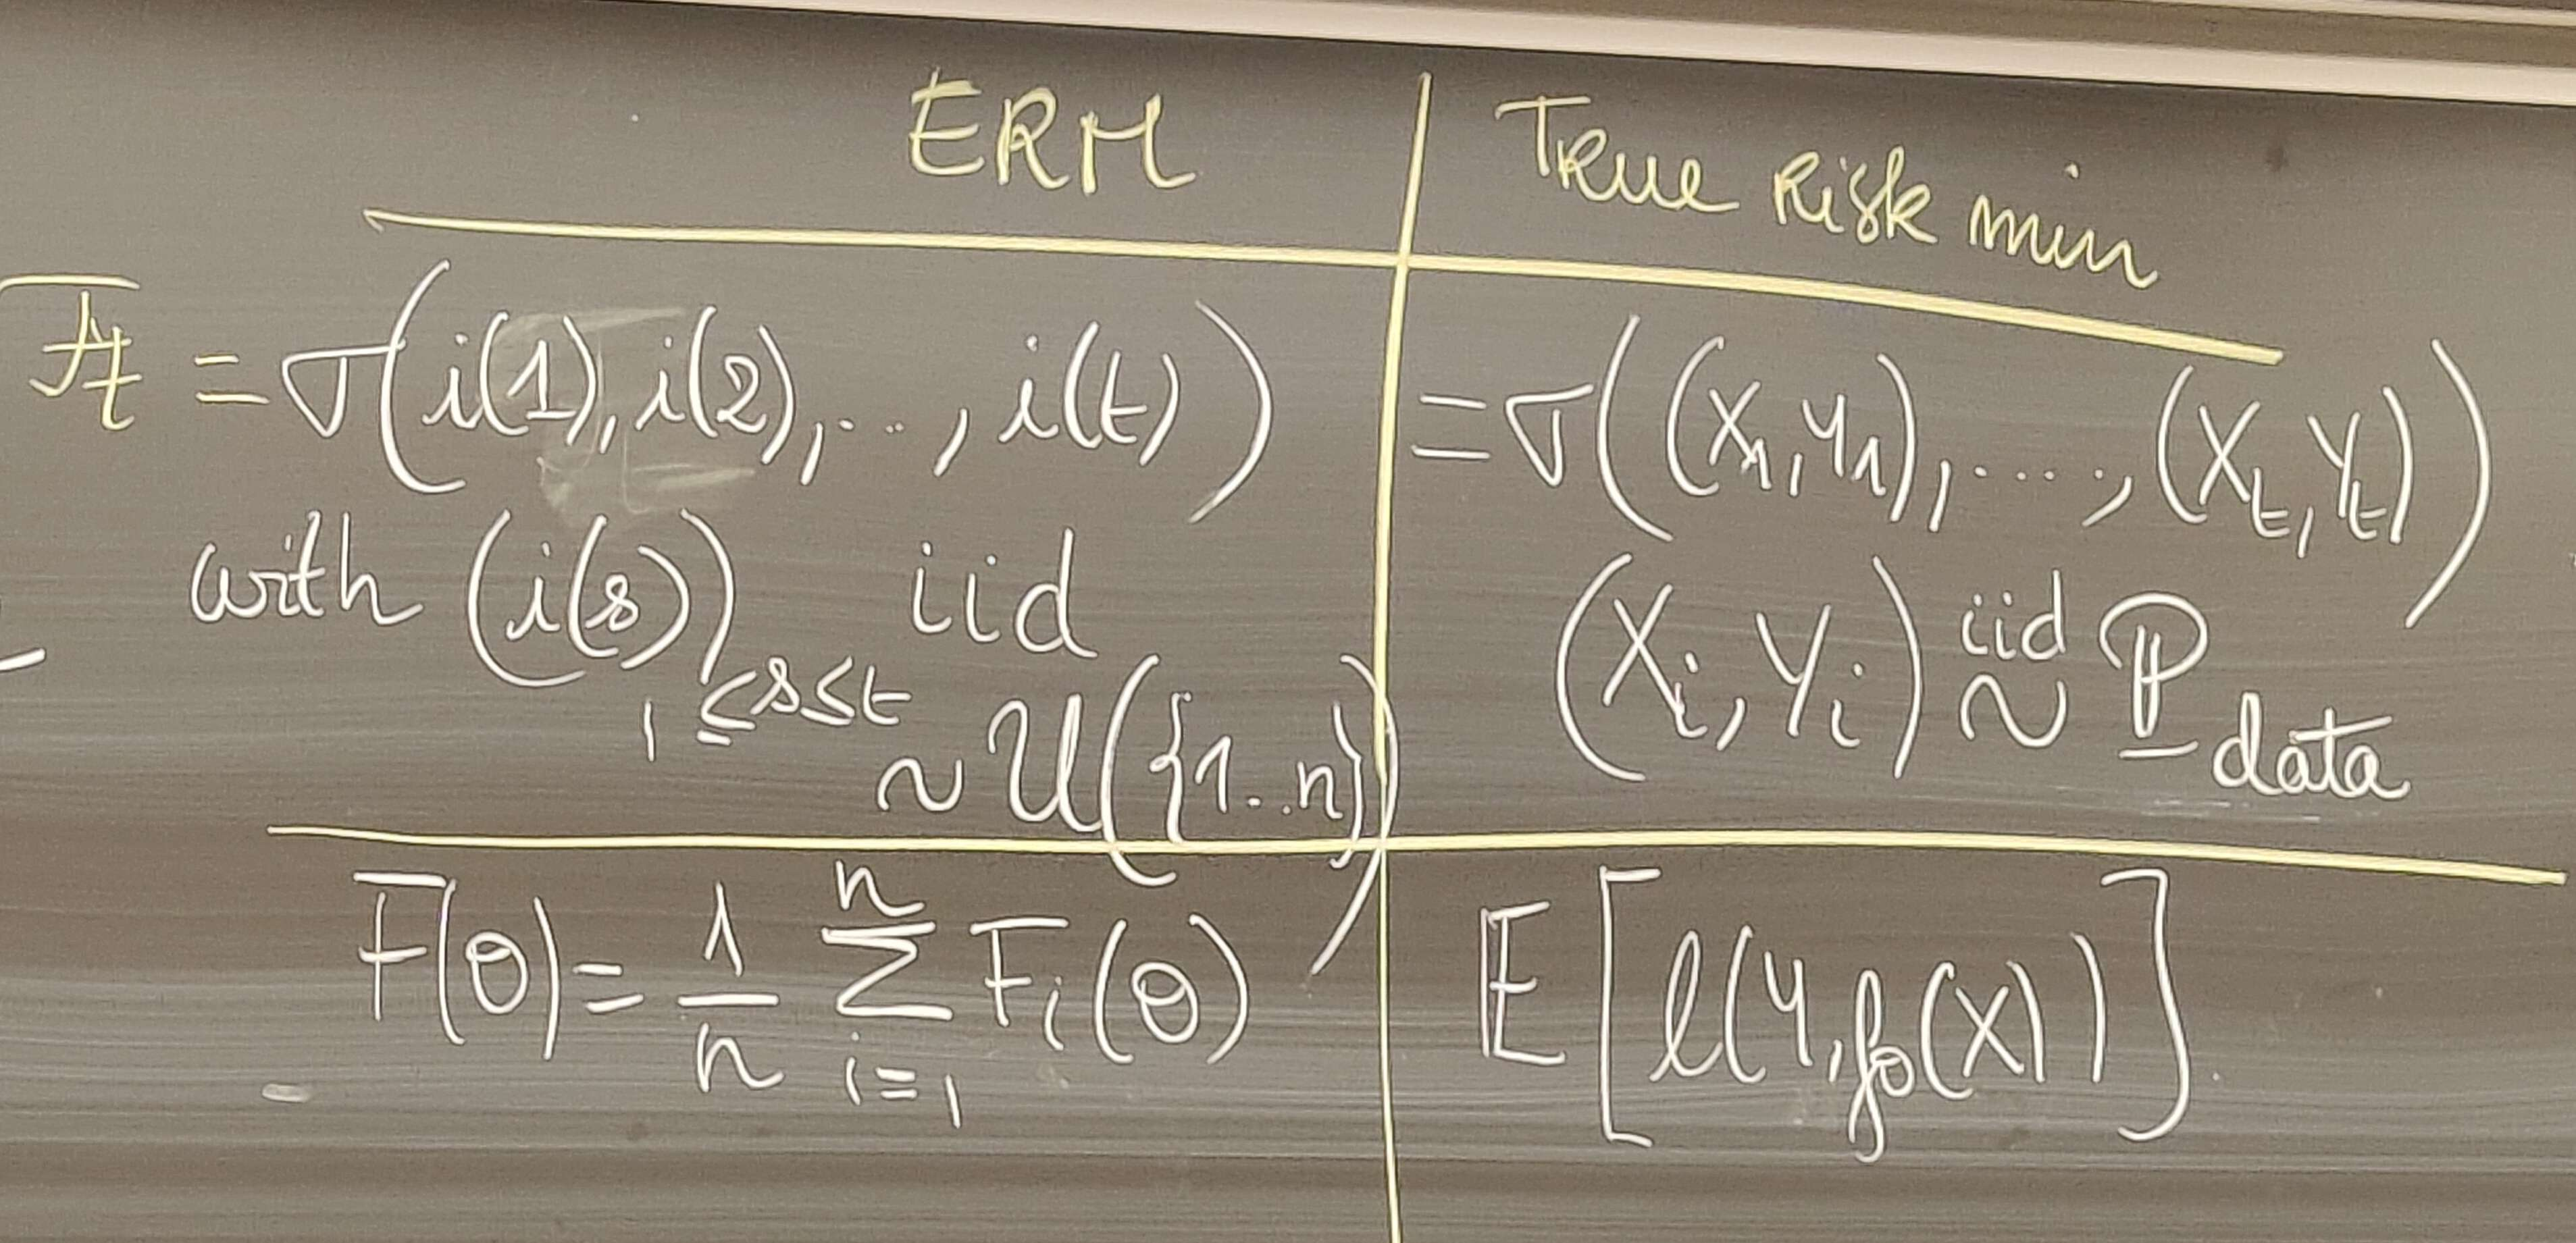
\includegraphics[width=.5\textwidth]{figs/thm_F_t.jpg}
    \caption{More explaination of $ \mathcal{F}_t $ }
    \label{explaination}
\end{figure}

\begin{note}
    \begin{itemize}
        \item 2 terms \begin{itemize}
            \item optimization term$\frac{\left\| \theta _0 - \theta ^\star  \right\|  ^2}{ 2 \gamma ( 1 - \frac{\gamma ^2}{2} ) T }$ similar to that of GD int the smooth case 
            \item The variance term $ \frac{\gamma  \sigma ^2}{2} $ impact of the noise which increase with $ \gamma  $ and $ \sigma ^2 $ 
        \end{itemize}
        
        \item Behaviour w.r.t $ \gamma  $ \begin{itemize}
            \item Because of optimisation : $ \frac{\left\| \theta _0 - \theta ^\star  \right\|  ^2}{ 2 \gamma ( 1 - \frac{\gamma ^2}{2} ) T } $ it goes up
            \item Bacause of Variance term : $ \frac{\gamma  \sigma ^2}{2} $ it goes down
        \end{itemize}
        
        \item Best trade-off is for $ \gamma \approx \frac{\left\| \theta _0 - \theta ^\star  \right\| }{4L \sqrt[]{T} \sigma } $ (constant step size but depending on the finit horizon)
        \item Comment the assumptions in the case ERM 
        \[
            F(\theta ) = \frac{1}{n} \sum_{i=1}^{n} F_i(\theta )
        .\]
        (ii) is satisfied whenever $ \forall t \geq 1, g_t = \nabla F_{i(t)} $ with $ i(t) \sim \mathcal{U}(\{1, \dots, n\})  $. \\
        Assume that (iii) holds for $ g_t = \nabla F_{i(t)} $ (usual SGD). \\
        One my use as gradient estimates $ g_t^{\left| B \right| } = \frac{1}{\left| B \right| } \sum_{i \in B_t} \nabla F_i$ where $ B_t $ is of cardinality $ \left| B_t \right| = \left| B \right|  $ uniformly ddrawn at random in $ \{ 1, \dots, n \} $  \\
        This is called a  \textbf{mini batch strategy}
        \begin{align*}
            \mathbb{E} [\left\| g_t^{\left| B \right| } (\theta ) - \nabla F(\theta)  \right\| ^2_2| \mathcal{F}_{t-1} ]
                &= \mathbb{E}[ \left\| \frac{1}{\left| B \right| } \sum_{i \in B_t}^{} \nabla F_i (\theta )  \right\| _2 ^2 | \mathcal{F}_{t-1} ] \\
                &= \mathbb{E}[ \left\| \frac{1}{\left| B \right| } \sum_{i \in B_t}^{} ( \nabla F_i (\theta ) - \nabla F(\theta )) \right\| _2 ^2 | \mathcal{F}_{t-1}] \\
                &= \frac{1}{\left| B \right|^2 } \left| B \right| \sigma ^2 = \frac{\sigma ^2}{\left| B \right| }
        \end{align*}
    \end{itemize}
\end{note}

\begin{proof}
    \[
        \left\| \theta _{t+1} - \theta ^{\star } \right\|^2_2 = \left\| \theta _{t} - \theta ^{\star } \right\|^2 - 2 \gamma _t \left\langle g_{t+1 }(\theta _t), \theta _t - \theta ^\star  \right\rangle + \gamma _t ^2 \left\| g_{t+1}(\theta _t) \right\| _2 ^2
    .\]
    Appying $ \mathbb{E}[ -1 \mathcal{F}_t] $ gives 
    \[
        \mathbb{E}[\left\| \theta _{t+1} - \theta ^\star  \right\| _2 ^2 | \mathcal{F}_t] = \left\| \theta _t - \theta ^\star  \right\| _2 ^2 - \mathbb{E}[2 \gamma _t \left\langle \nabla F(\theta _t), \theta _t - \theta ^\star  \right\rangle | \mathcal{F}_t] + \gamma _t ^2 \mathbb{E}[ \left\| g_{t+1} (\theta _t) \right\| _2 ^2 | \mathcal{F}_t]
    .\]
    $\left\| \theta _t - \theta ^\star  \right\| _2 ^2$ is $\mathcal{F}_t$-mesurable. and $\mathbb{E}[-2 \gamma _t \left\langle \nabla F(\theta _t), \theta _t - \theta ^\star  \right\rangle | \mathcal{F}_t] = -2 \gamma _t \left\langle \mathbb{E}[\nabla F(\theta _t)| \mathcal{F}_t], \theta _t - \theta ^\star  \right\rangle  = -2 \gamma _t \left\langle g_{t+1 }(\theta _t), \theta _t - \theta ^\star  \right\rangle  $ as $\theta _t - \theta ^\star  $ is $\mathcal{F}_t$-mesurable and with (ii).
    
    
    \begin{align*}
        \gamma _t ^2 \mathbb{E}[ \left\| g_{t+1} (\theta _t) \right\| _2 ^2 | \mathcal{F}_t] 
            &= \gamma _t ^2 \mathbb{E}[ \left\| g_{t+1} (\theta _t) - \nabla F(\theta _t) + \nabla F(\theta _t) \right\| _2 ^2 | \mathcal{F}_t ] \\
            &= \gamma _t ^2 \mathbb{E} [ \left\| g_{t+1}(\theta _t) - \nabla F(\theta _t) \right\| _2 ^2 | \mathcal{F}_t ] + \gamma _t ^2 \left\| \nabla F(\theta _t) \right\| _2 ^2 + 2 \gamma _t ^2 \left\langle \mathbb{E}[g_{t+1}(\theta _t) | \mathcal{F}_t ] - \nabla F(\theta _t), \nabla F(\theta _t) \right\rangle \\
            &= \gamma _t ^2 \mathbb{E} [ \left\| g_{t+1}(\theta _t) - \nabla F(\theta _t) \right\| _2 ^2 | \mathcal{F}_t ] + \gamma _t ^2 \left\| \nabla F(\theta _t) \right\| _2 ^2 + 2 \gamma _t ^2  * 0 \text{ not sure it's what she mean}\\
            &\leq \gamma _t ^2 \sigma ^2 + \gamma _t \left\| \nabla F (\theta _t) \right\| _2 ^2 \\
            &\leq \gamma _t ^2 \sigma ^2 + \gamma _t ^2 L \left\langle \nabla F(\theta _t) , \theta _t - \theta ^\star  \right\rangle \\
            & \text{ by cocoercivity of the gradient } \nabla F
    \end{align*}
    We get 
    \[
        \mathbb{E}[ \left\| \theta _{t+1} - \theta ^\star  \right\| _2 ^2 | \mathcal{F}_t] \leq \left\| \theta _t - \theta ^\star  \right\| _2 ^2 + ( -2 \gamma _t + \gamma _t ^2 L ) \left\langle \nabla F(\theta _t) , \theta _t - \theta ^\star  \right\rangle + \gamma _t ^2 \sigma ^2
    .\]
    By convexity of $ F $, 
    \begin{align*}
        F(\theta ^\star ) &\geq F(\theta e_t) + \left\langle \nabla F(\theta _t)  , \theta ^\star - \theta _t \right\rangle \\
        \text{i.e. } F(\theta _t) F^\star &\leq \left\langle \nabla F(\theta _t) , \theta _t - \theta ^\star  \right\rangle 
    \end{align*}
    If $ \gamma _t = \gamma \leq 1/L $, then 
    \begin{align*}
        0 \leq  \gamma _t L \leq 1 \\
        -2 \leq  -2 + \gamma _t L \leq  -1 \\
        -2 \gamma _t + \gamma _t ^2 L \leq - \gamma _t
    \end{align*}
    Therefore 
    \[
        \gamma \mathbb{E}[ F(\theta _t ) - F^\star ] \leq \mathbb{E}b[ \left\| \theta _t - \theta ^\star  \right\| _2 ^2] - \mathbb{E} [ \left\| \theta _{t+1} - \theta ^\star  \right\| _2 ^2 ] + \gamma ^2 \sigma ^2
    .\]
    Using Jensen's inequality, $ F(\bar{\theta _T}) = \frac{1}{\gamma T} \sum_{t=1}^{T} F(\theta _t) $. \\   
    Finaly 
    \[
        \mathbb{E}[F (\bar{\theta }_T - F^\star )] \leq \frac{1}{T}\sum_{t=1}^{T}\mathbb{E}[F(\theta _t) - F^\star ] \leq \frac{1}{\gamma T} \left\| \theta _0 - \theta ^\star  \right\| _2 ^2 + \gamma ^2 \sigma ^2
    .\]
\end{proof}
\begin{thm}[]
    F $\mu$-strongly cvx $L$-smooth. Ball $"\kappa = L/ \mu "$ \\
    Choose $\gamma _t = \begin{cases}
        \frac{1}{2L} &\text{ for } t \leq 4 \left\lceil \kappa  \right\rceil \\
        \frac{2t+1}{(t+1)^2 \mu} &\text{ for } t > 4 \left\lceil \kappa  \right\rceil \\
    \end{cases} $

    If $ t \geq 4 \left\lceil \kappa \right\rceil  $ , then 
    \[
        \mathbb{E}[\left\| \theta _t - \theta ^\star  \right\| _2 ^2 ] \leq \frac{\sigma ^2 4}{\mu t} + \frac{16 \left\lceil \kappa  \right\rceil ^2 }{c t^2} \left\| \theta _0 - \theta ^\star  \right\| _2 ^2
    .\]
    
\end{thm}

\begin{proof}[Proof:]
    See [Gower. ] 2014 / 2016. 
    
    TD : In the case $ \mu  $ -strongly convex \begin{itemize}
        \item $ \gamma = \frac{2}{\mu (t+1)} $
        \item $ \left\| g_t (\theta ) \right\| \leq b $  a.s. $ \forall \theta  $ 
        \item $ \theta _t = proj_B (\theta _{t-1} - \gamma _t g_t (\theta _{t-1})) $ 
    \end{itemize}
\end{proof}

\begin{note}[]
    \begin{itemize}
        \item \textbf{Good: } The result hold for the objective fonction 
        \[
            F(\theta ) - F(\theta ^\star ) \leq \left\langle \nabla F(\theta ^\star ), \theta - \theta ^\star  \right\rangle  + \frac{L}{2} \left\| \theta - \theta ^\star  \right\| _2 ^2 
        .\]
        \[
            \mathbb{E}[\left\| \theta _t - \theta ^\star  \right\| _2 ^2] = O(1/t) \Rightarrow \mathbb{E}[F(\theta _t) - F^\star ] = O(1/t)
        .\]
        
        \item \textbf{Bad: } With this proof strategy, we do not see the benefit of P-R averaging
        \[
            \mathbb{E}[F ( \bar{\theta}_T ) - F^\star ] \leq \frac{1}{T} \mathbb{E}[ \sum_{t=1}^{T} F(\theta _t) - F^\star ] \leq 0(\frac{\log_{} T  }{T})
        .\]
    \end{itemize}
\end{note}

We have proven this 
\begin{thm}[]
    $F$ smooth, unbiased gradients, uniformly bounded variance    
    \[
        \mathbb{E}[F(\bar{\theta }_T) - F^\star ] \leq \frac{\left\| \theta _0 - \theta ^\star  \right\| _2 ^2 }{\gamma T} + \gamma \sigma ^2 
    .\]
    For $ \gamma \propto 1 / \sqrt[]{T} $ 
    \[
        = O (1 / \sqrt[]{T})
    .\]
\end{thm}

\[
    \mathbb{E}[F({\theta }_t) - F^{\star} ] \leq \frac{1}{\gamma T} \left\| \theta _0 - \theta^{\star } \right\|^2 + \gamma  \sigma ^2 
.\]


\paragraph*{Exercice}
TD : In the case $ \mu  $ -strongly convex \begin{itemize}
    \item $ \gamma = \frac{2}{\mu (t+1)} $
    \item $ \left\| g_t (\theta ) \right\| \leq b $  a.s. $ \forall \theta  $ 
    \item $ \theta _t = proj_B (\theta _{t-1} - \gamma _t g_t (\theta _{t-1})) $ 
\end{itemize}

\paragraph*{Exercice 1 - TD3}
\begin{enumerate}
    \item \begin{align*}
        \left\| \theta _t - \theta ^\star  \right\| _2 ^2 
            &= \left\| proj_B (\theta _{t-1} - \gamma _t g_t (\theta _{t-1})) - \theta ^\star  \right\| _2 ^2 \\
            &= \left\| proj_B (\theta _{t-1} - \gamma _t g_t (\theta _{t-1})) - proj_B(\theta ^\star ) \right\| _2 ^2 \\
            &\leq \left\| \theta _{t-1} - \gamma _t g_t(\theta _{t - 1}) - \theta ^\star \right\| _2 ^2 \\
            &= \left\| \theta _t - \theta  ^\star  \right\| _2 ^2 + \gamma _t ^2 \left\| g_t(\theta _{t-1}) \right\| _2 ^2 - 2 \gamma _t \left\langle g_t(\theta _{t-1}), \theta _{t-1} - \theta ^\star  \right\rangle \\
        \mathbb{E}[ \left\| \theta _t - \theta ^\star  \right\| _2 ^2 | \mathcal{F}_{t-1}] 
            &\leq \mathbb{E}[\left\| \theta _{t-1} - \theta ^\star  \right\| _2 ^2 + \gamma _t ^2 \left\| g_t (\theta _{t-1} ) \right\| _2 ^2 - 2 \gamma _t \left\langle g_t(\theta _{t-1} ), \theta _{t-1} - \theta ^\star  \right\rangle | \mathcal{F}_{t-1}]
            &\leq \left\| \theta _{t-1} - \theta ^\star  \right\| _2 ^2 + \gamma _t ^2 b^2 - 2 \gamma _t \left\langle \nabla F(\theta _{t-1}), \theta _{t-1} - \theta ^{\star } \right\rangle 
    \end{align*}
    
    \item By $ \mu  $ - strong convex, $ F(y) - F(x) \geq \left\langle \nabla F(x) , y - x \right\rangle + \frac{\mu }{2} \left\| y - x \right\| _2 ^2, \forall x,y  $ \\
    for $x = \theta_{t-1}$ and $y = \theta ^{\star }$,
    
    \[
        F(\theta_{t-1}) - F(\theta ^{\star }) \leq \left\langle \nabla F(\theta_{t-1}) , \theta_{t-1} - \theta ^{\star } \right\rangle + \frac{\mu }{2} \left\| \theta_{t-1} - \theta ^{\star } \right\| _2 ^2
    .\]
    \begin{enumerate}
        \item $ \leq \frac{1}{2 \gamma _t } \left\| \theta _{t-1} - \theta ^\star  \right\| _2 ^2 + \frac{\gamma + b^2}{2} - \frac{1}{2 \gamma _t} \mathbb{E}[ \left\| \theta _t - \theta  ^\star  \right\| _2 ^2 | \mathcal{F}_{t-1}] - \frac{\mu }{2} \left\| \theta _{t-1} - \theta ^\star  \right\| _2 ^2 $ 
        \begin{align*}
            \mathbb{E}[F(\theta _{t-1} - F(\theta ^\star ))] 
                &\leq \frac{\mu (t+1)}{4} \mathbb{E}[\left\| \theta _{t-1} - \theta ^\star  \right\| ^2 ] + \frac{b^2}{ \mu (t+1)} - \frac{\mu (t+1)}{4} \left\| \theta _t - \theta ^star \right\| ^2 - \frac{\mu }{2} \mathbb{E}[\left\| \theta _{t-1 - \theta ^\star } \right\|^2] \\
            \mathbb{E}[F(\theta _{t-1}) - F(\theta ^\star )] 
                &\leq \frac{\mu (t-1)}{4} \mathbb{E}[\left\| \theta _{t-1} - \theta  ^\star  \right\|^2 ] - \frac{\mu (t+1)}{4} \mathbb{E}[\left\| \theta _t - \theta  ^\star  \right\| ^2 ] + \frac{b^2}{\mu (t+1)} \\
            \sum_{s=1}^{t}s \mathbb{E}[F(\theta _{s-1}) - F(\theta ^\star )] 
                &\leq \frac{\mu }{4} [\sum_{s=1}^{t} s (s-1) \mathbb{E}[\left\| \theta _{s-1} - \theta ^\star  \right\| _2 ^2] - s(s-1)\mathbb{E}[\left\| \theta _s - \theta ^\star  \right\| ^2]] + \frac{b^2}{\mu }t  \\
                &\leq \frac{b^2}{\mu }
        \end{align*}
        By convexity of F :
        \begin{align*}
            \mathbb{E}[F(\frac{2}{t(t+1)} \sum_{s=1}^{t} s \theta _{s-1}) - F(\theta ^{\star })] &\leq \frac{2}{t(t+1)} \sum_{s=1}^{t} s \mathbb{E}[F(\theta _{s-1}) - F(\theta ^{\star }) ]\\
            &\leq \frac{2}{t(t+1)} \sum_{s=1}^{t} s \mathbb{E}[F(\theta _{s-1}) - F (\theta ^\star )] \\
            &\leq \frac{2b^2}{\mu (t+1)}
        \end{align*}        
    \end{enumerate}
\end{enumerate}

\begin{note}[]
    \begin{itemize}
        \item L-smooth constant $ \gamma = mathcal{O}(1/\sqrt[]{T}) $, rate $ = mathcal{O}(1/\sqrt[]{T}) $ 
        \item L-smooth \& $ mu $-strongly convex, $ \gamma _t \propto \frac{1}{t} $ : rate $ = mathcal{O}(1/t) $ 
    \end{itemize}
    \begin{figure}[!h]
        \centering
        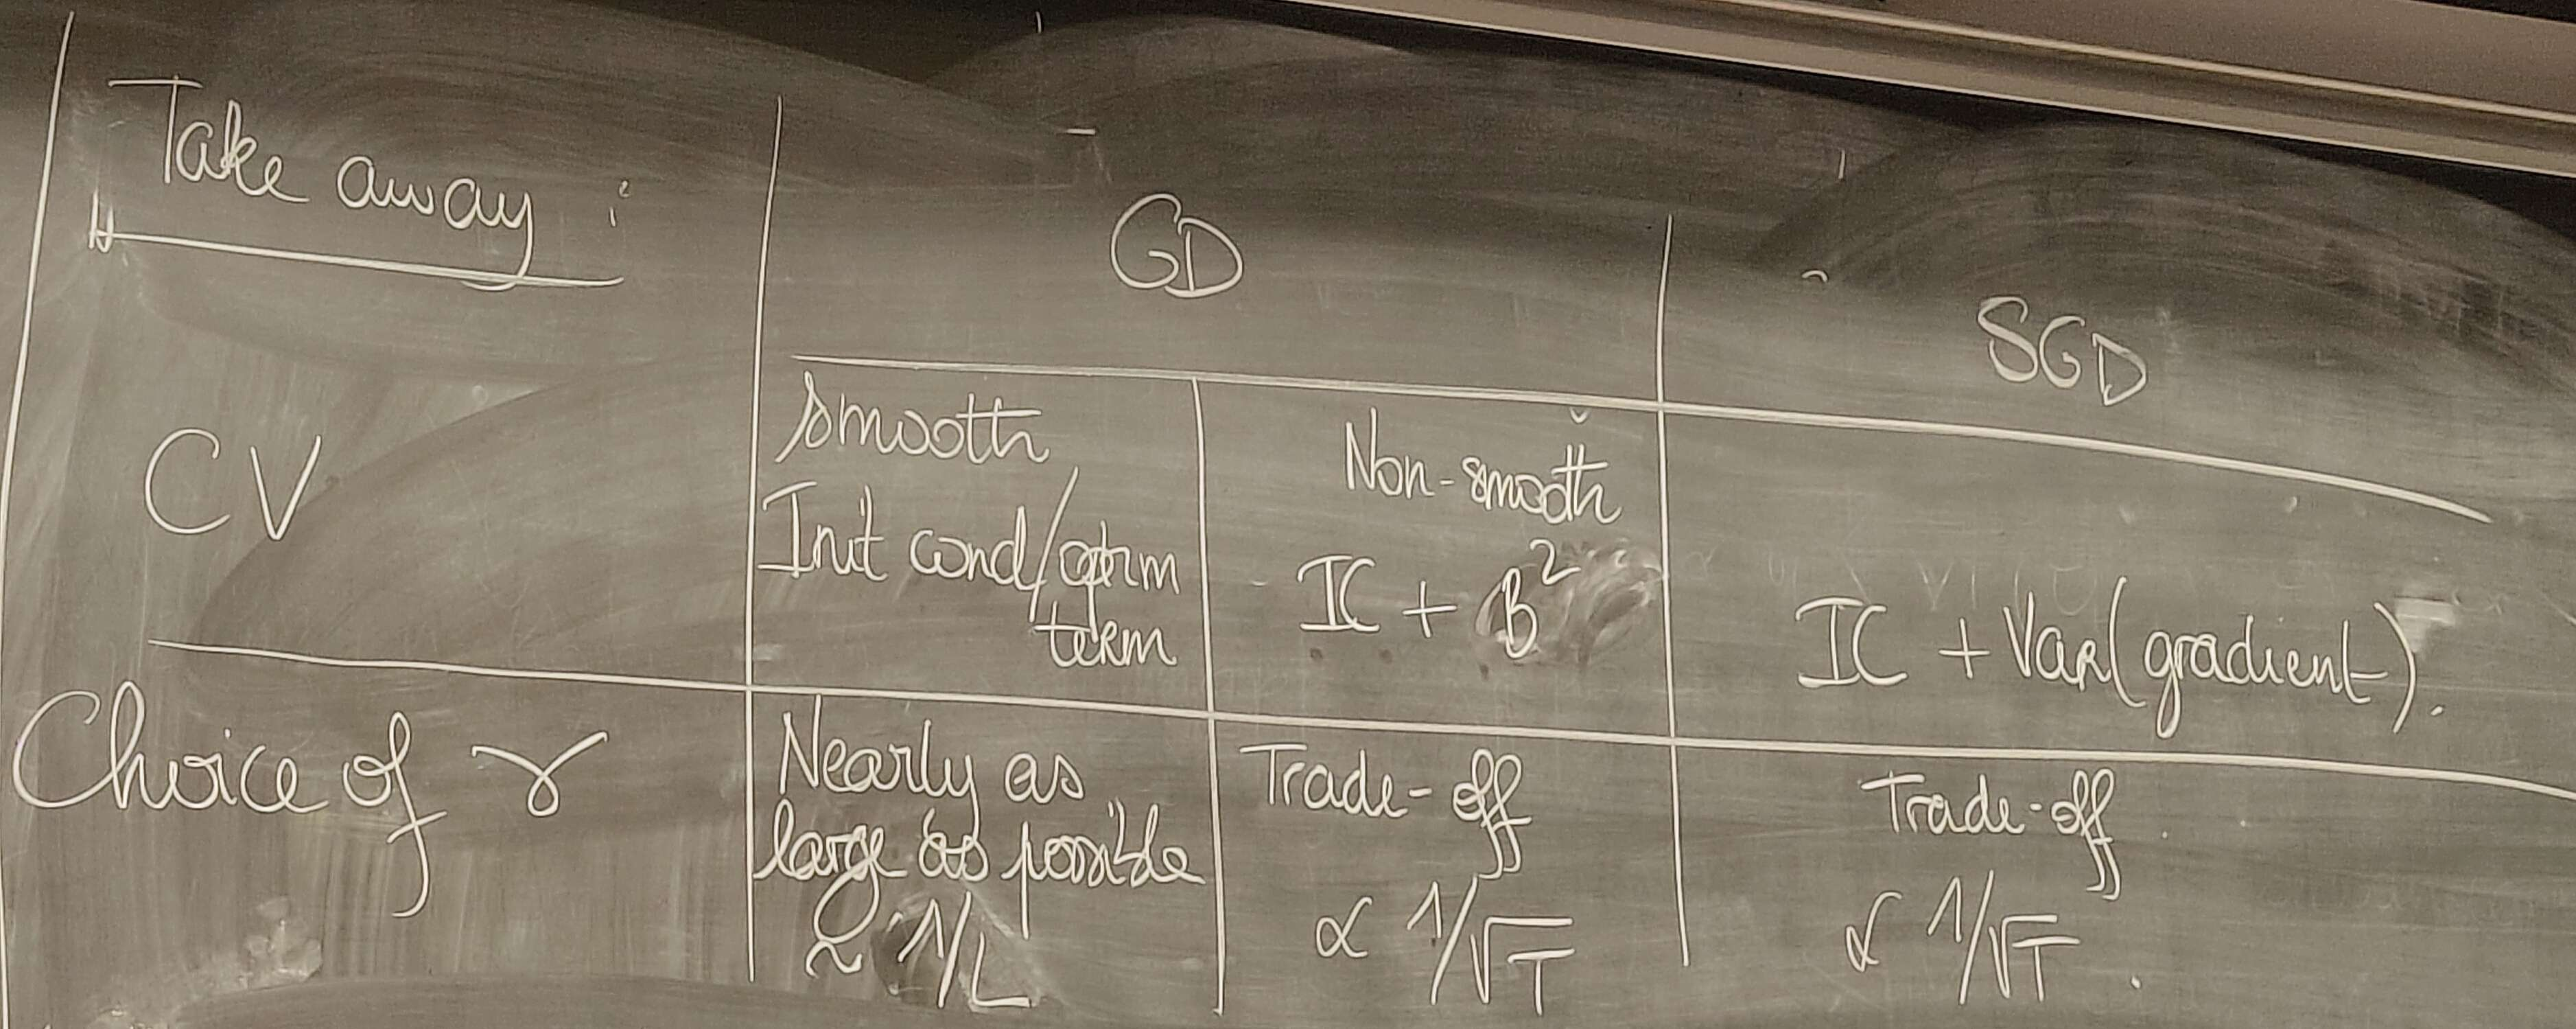
\includegraphics[width=.8\textwidth]{figs/take_away_table.jpg}
        \caption{Take Away table}
    \end{figure}

    \paragraph*{In terms of optimization, SGD vs GD : who is best?}
    Constext : $F$ smooth, ERM $F(\theta ) = \frac{1}{n} \sum_{i=}^{n} F_i(\theta )$
    \begin{figure}[!h]
        \centering
        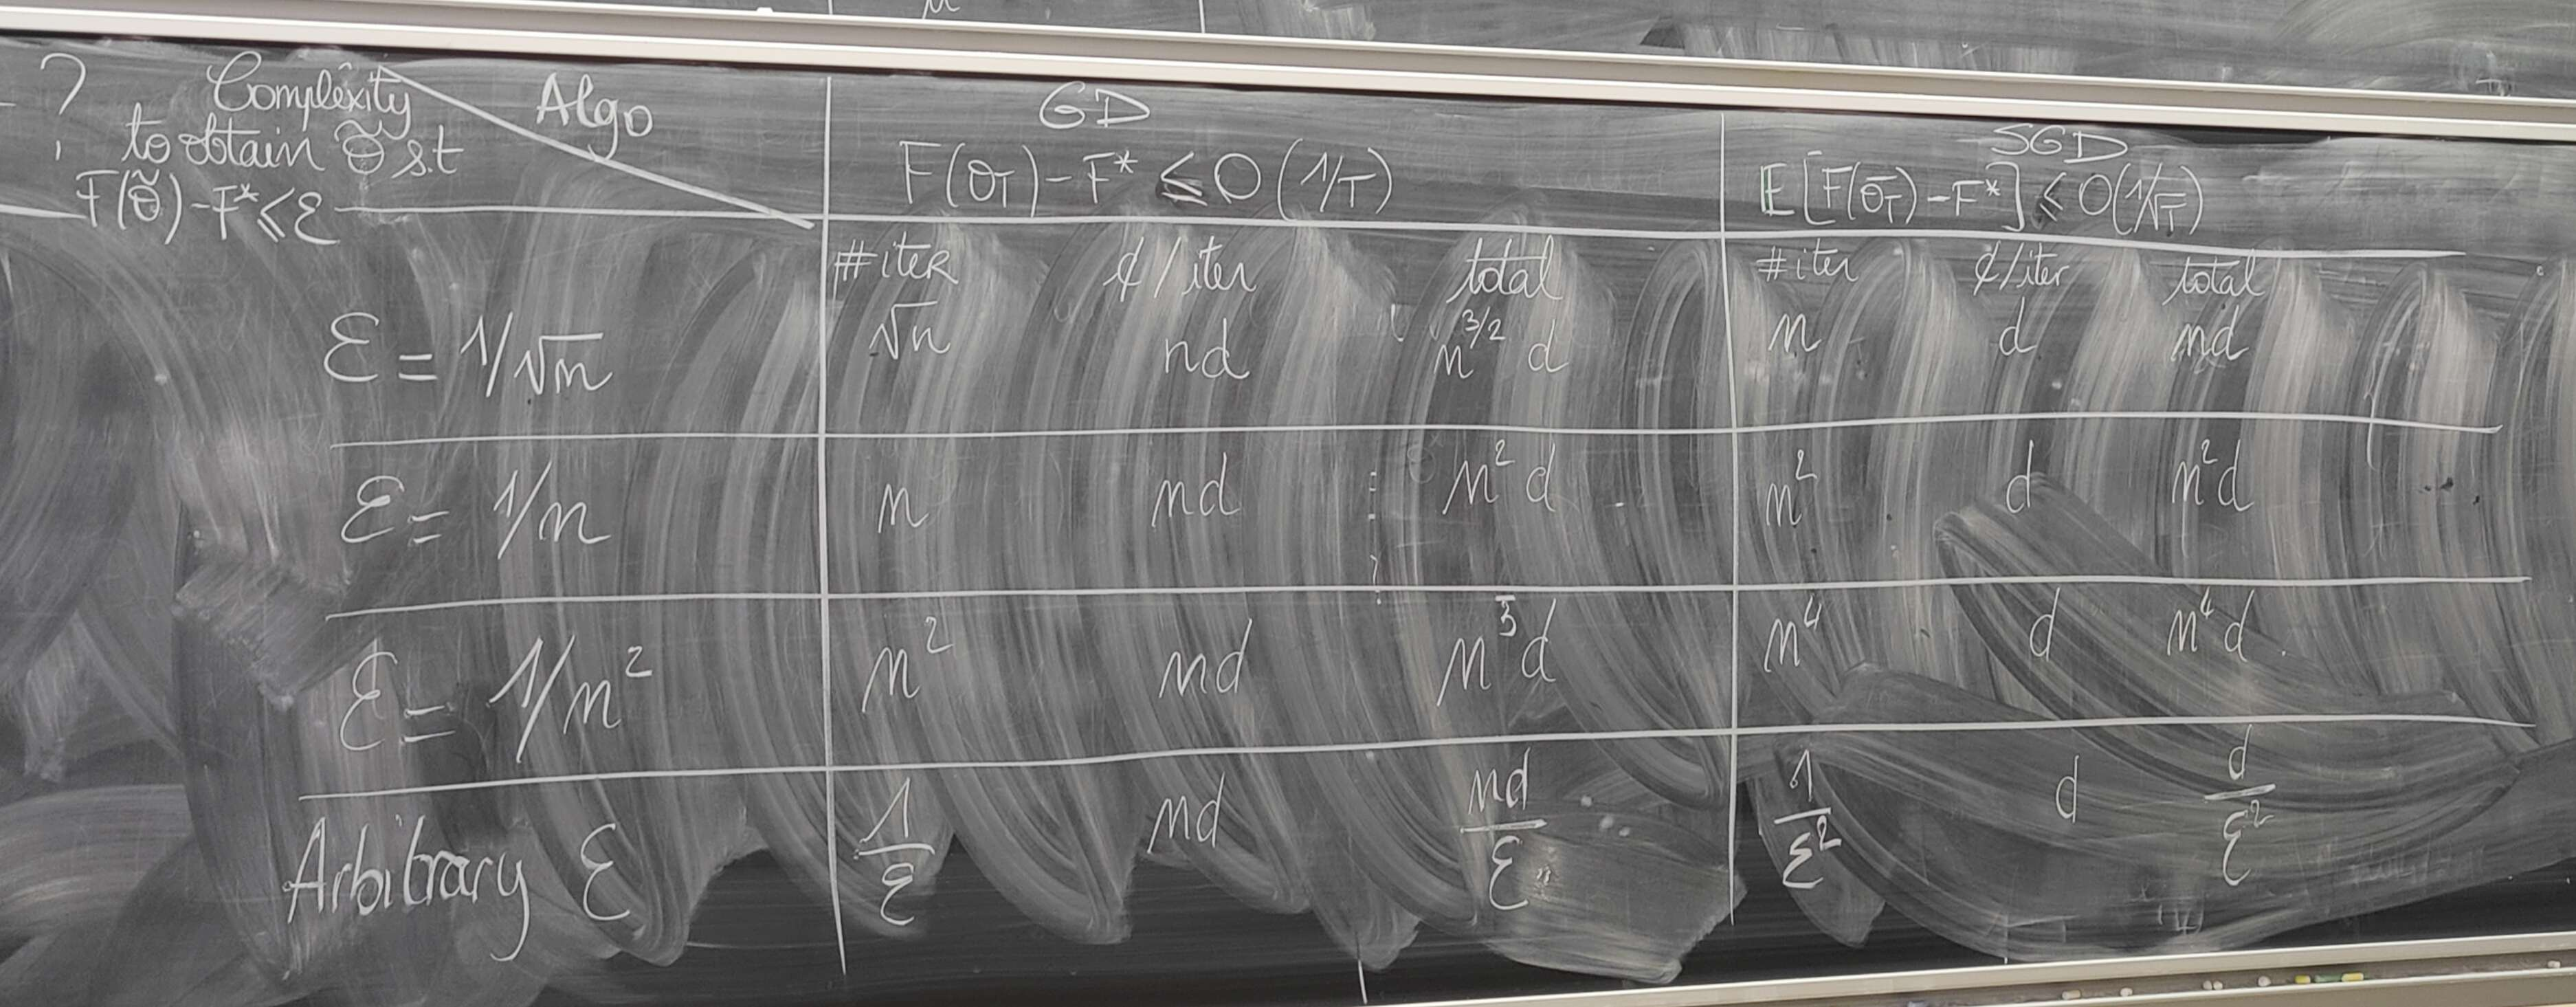
\includegraphics[width=.8\textwidth]{figs/SGD_vs_GD.jpg}
        \caption{In terms of optimization, SGD vs GD : who is best? }
    \end{figure}
    \begin{figure}[!h]
        \centering
        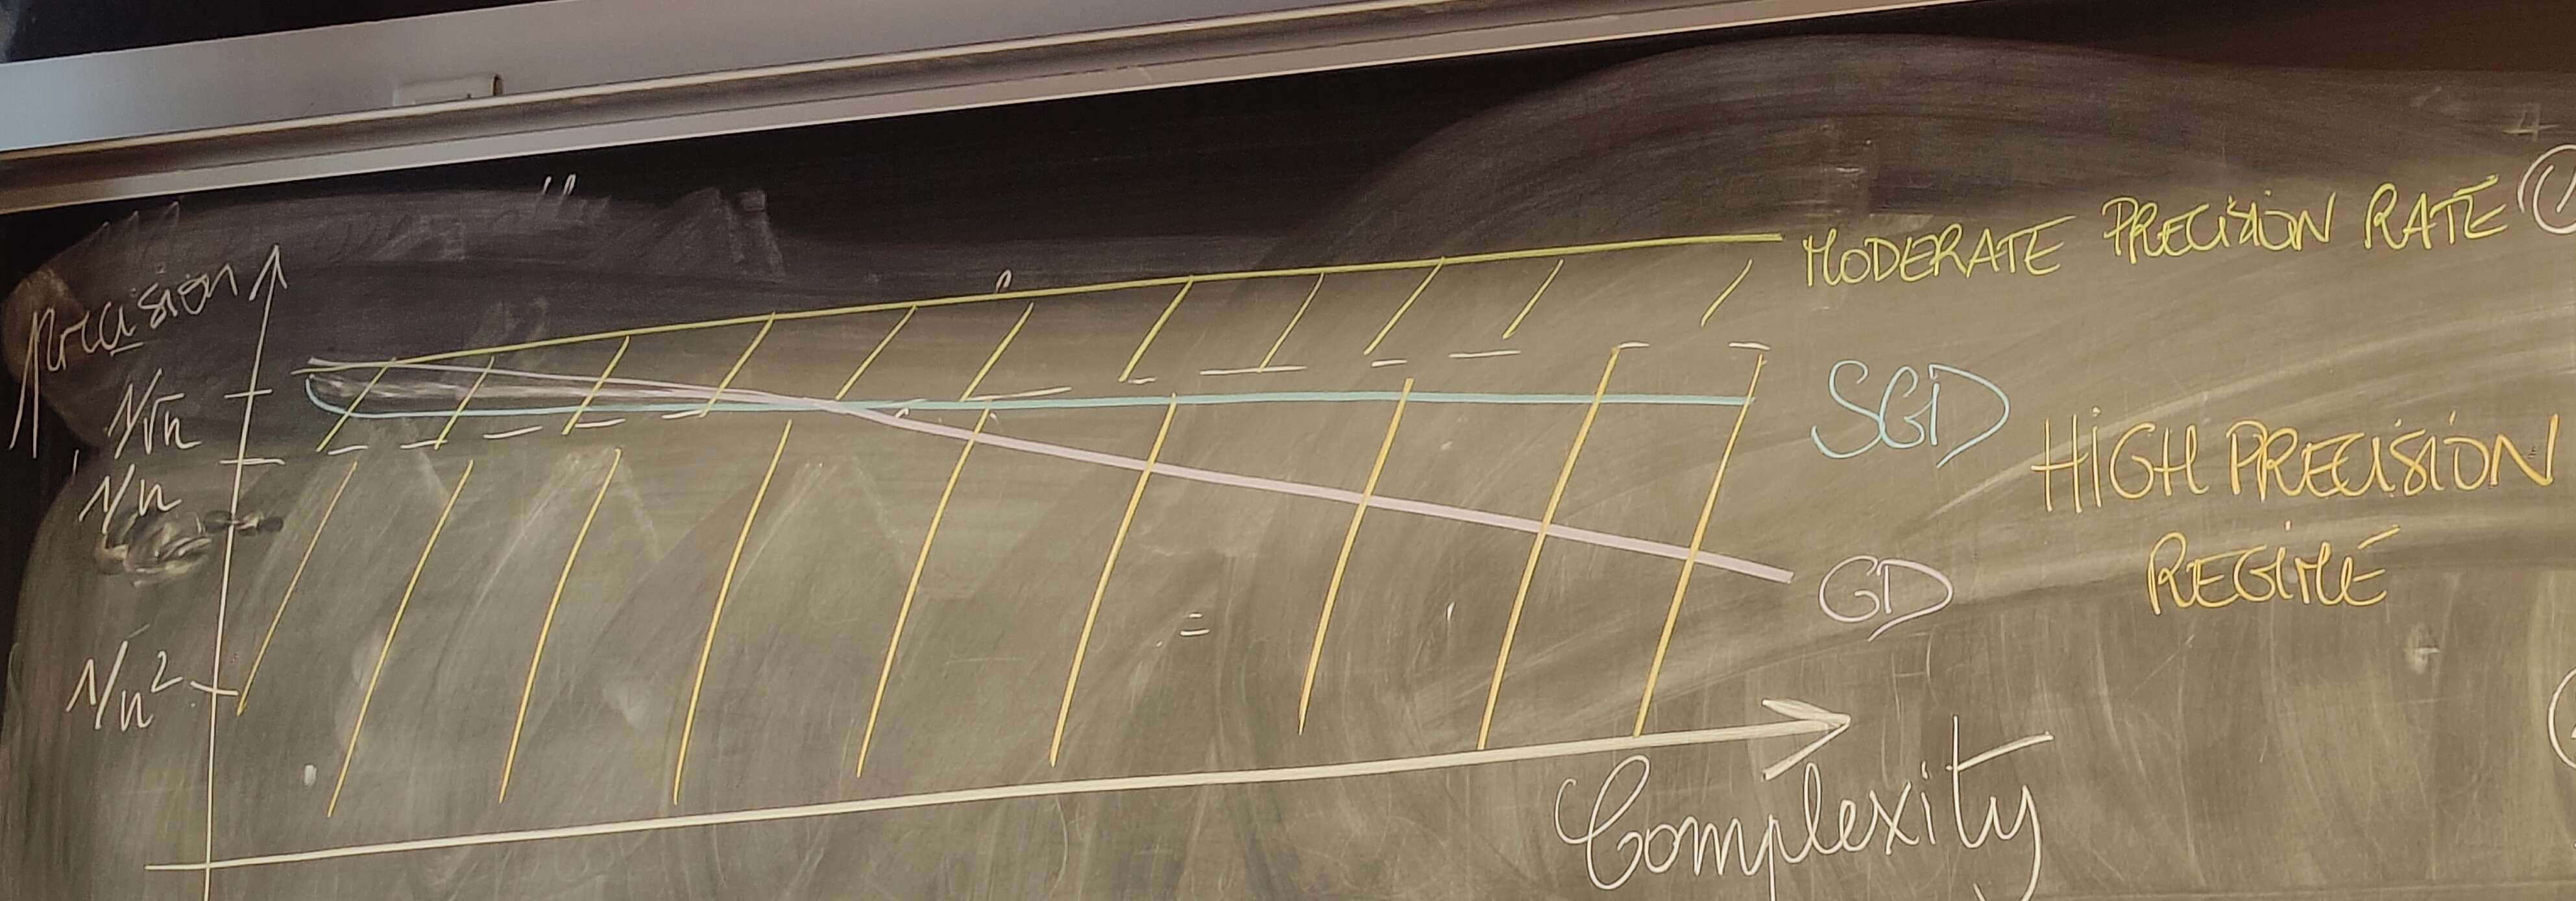
\includegraphics[width=.8\textwidth]{figs/SGD_vs_GD_graph.jpg}
        \caption{In terms of optimization, SGD vs GD : who is best? Graph }
    \end{figure}

    \begin{enumerate}
        \item GD tends to outperform SGD (in termes of complexity) for hig presion regimes
        \item SGD outperforms GD for low to moderate precision regimes
    \end{enumerate}
    So none is best. It depends to the precision. \\
    The frontier between "moderate" \& "high" precision has been fixed to $\frac{1}{n}$.
    In ML, one aims to optimize up to the \textbf{statistical} precision, ranging from $ 1 / \sqrt[]{n} $ to $ 1/n $, thus moderate precision is enough! \\
    
    \textbf{CCL}\begin{itemize}
        \item For optimization, no best method between GD and SGD
        \item For ML , moderate precision, better choose SGD
    \end{itemize}

    \paragraph*{In terms of generalization?}
    \begin{itemize}
        \item Running SGD for the expected risk minimization with $ n $ samples leads to a generatization error $ \propto 1/\sqrt[]{n} $. This has to be compared with classical bounds of stat/ML
        \begin{figure}[!h]
            \centering
            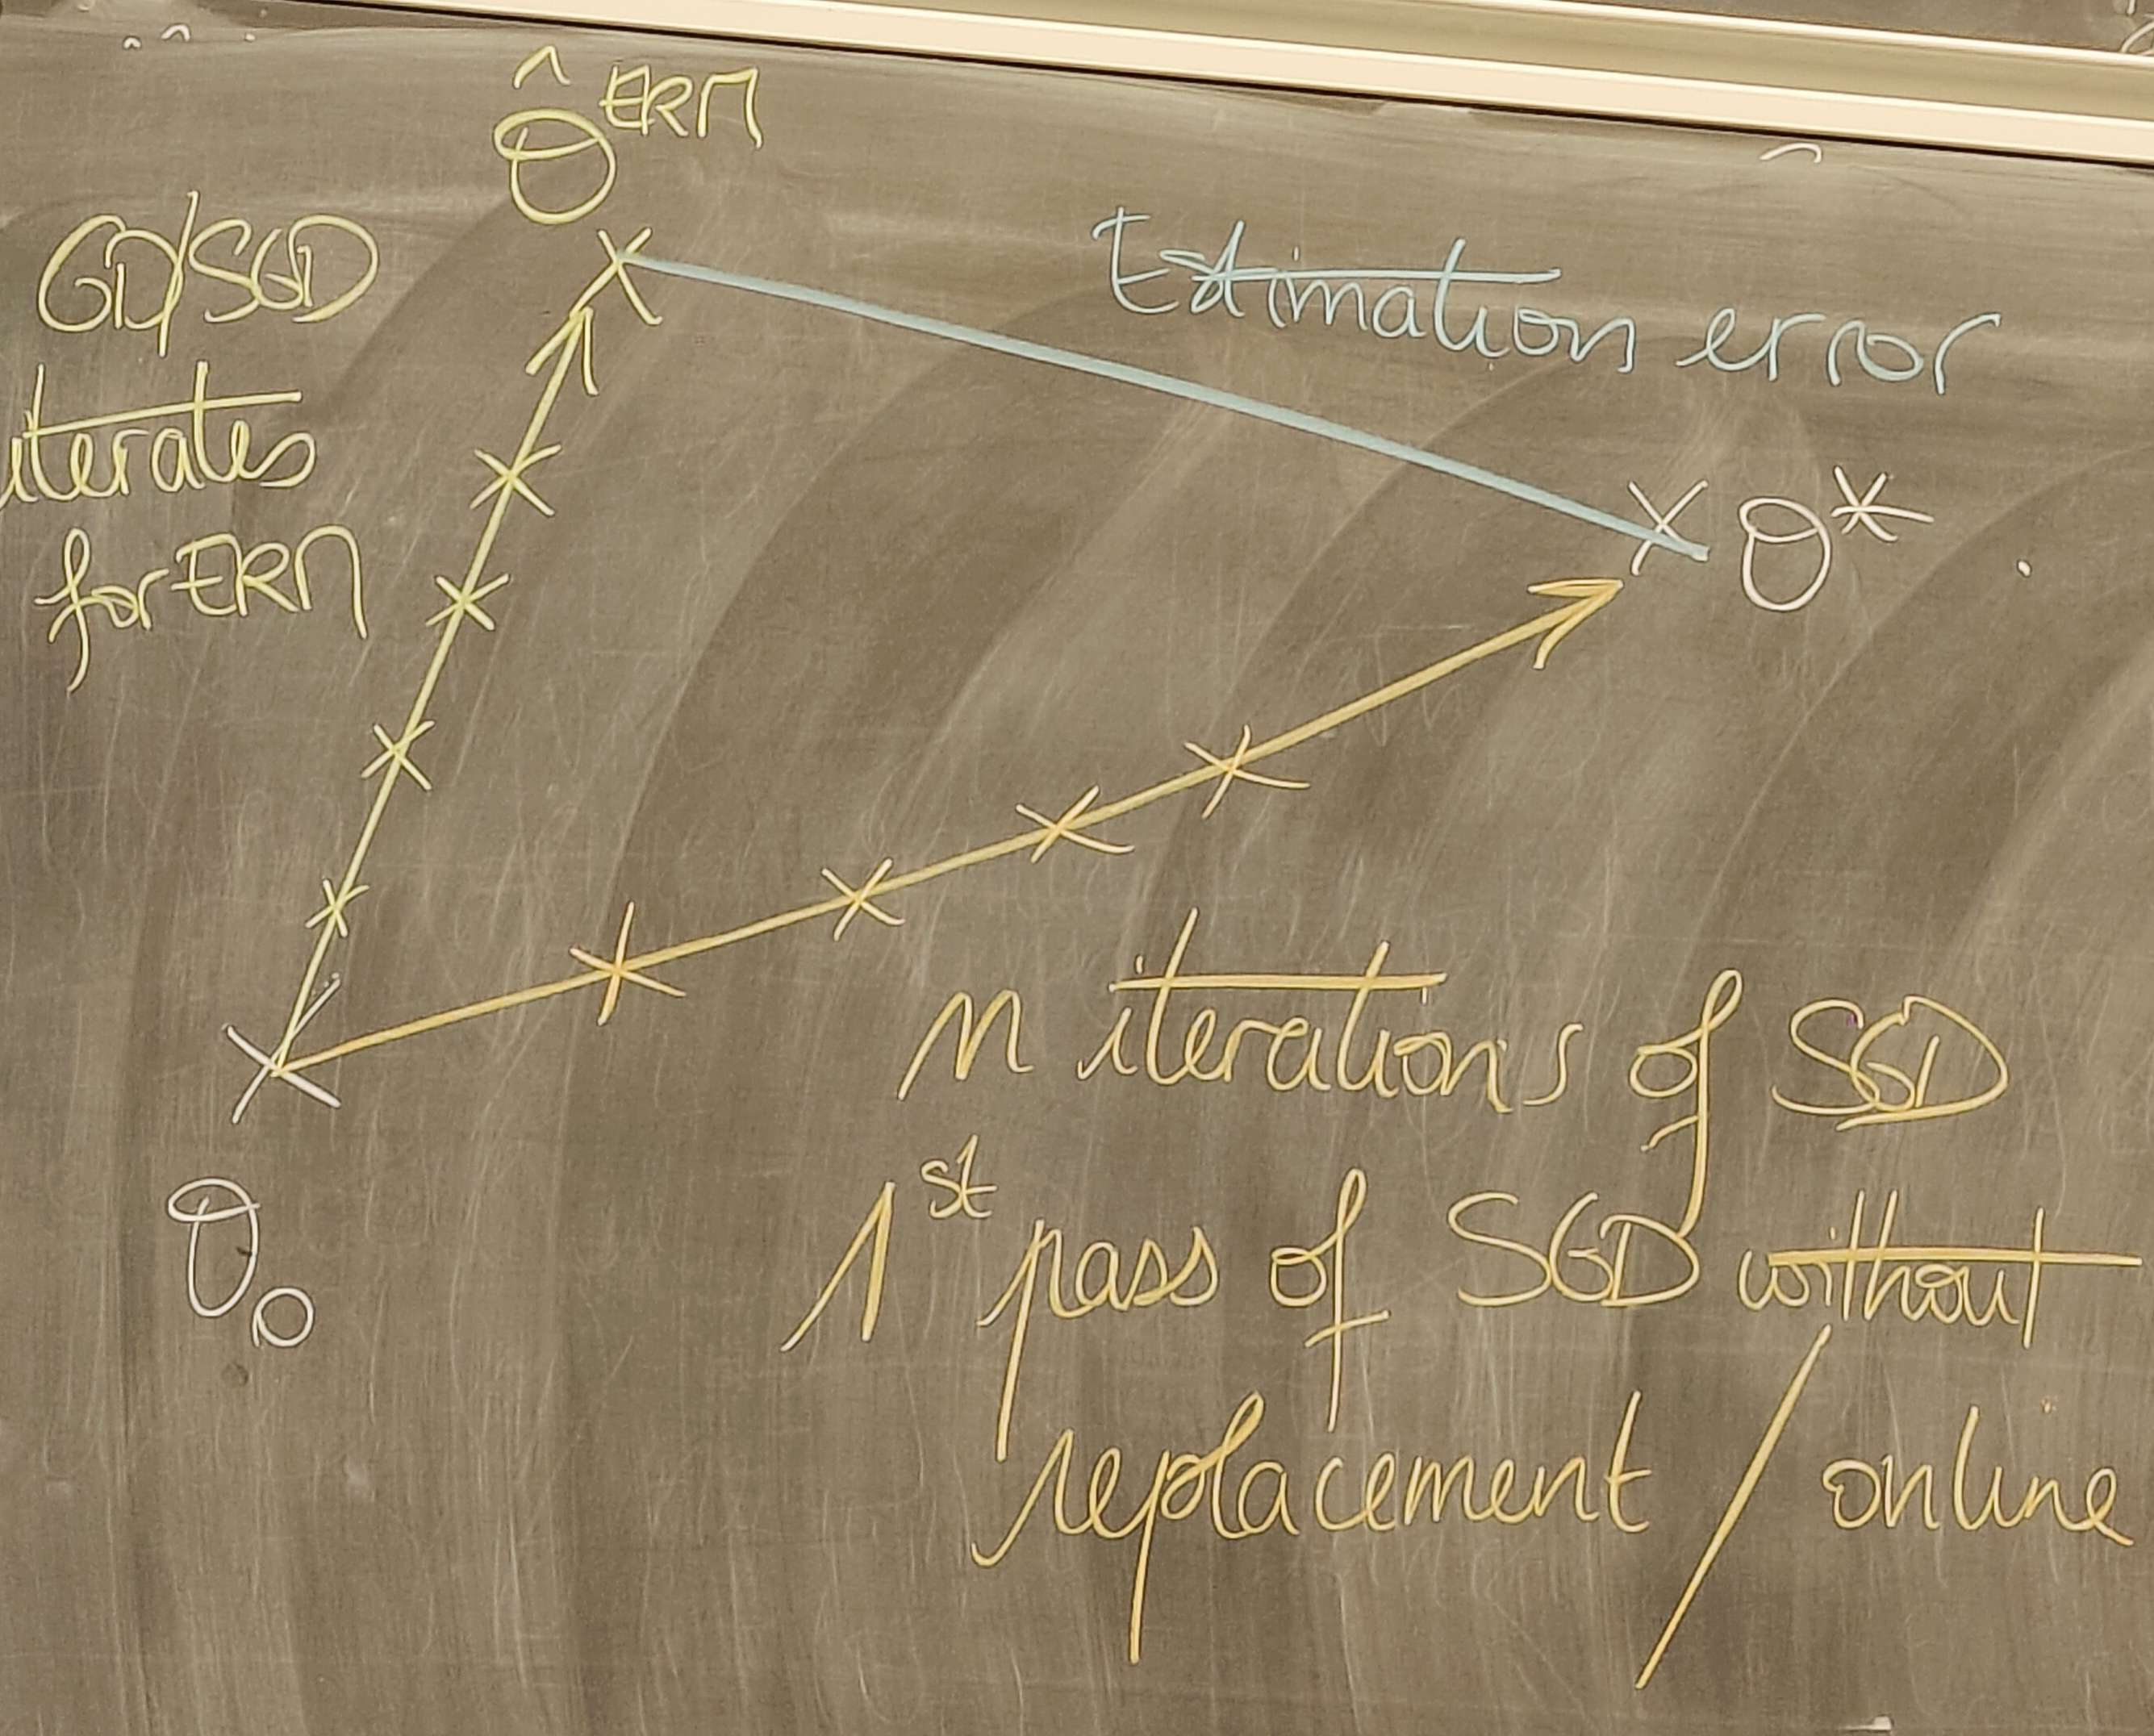
\includegraphics[width=.8\textwidth]{figs/SGD_vs_GD_generalization.jpg}
            \caption{In terms of optimization, SGD vs GD : who is best? Graph }
        \end{figure}
        SGD on the expected risk avoids estimation pb. One pass of SGD may be competitive without exact ERM. \\
        In term of running complexities, we get :
        \begin{align*}
            \mathcal{O} (tnd) = \mathcal{O}(n^2 d) &\text{ vs } \mathcal{O}(nd) \\
            (GD \text{ for } ERM) &\text{ vs } (SGD)
        \end{align*}
        \textbf{Warning} We are only comparing upperbounds!
        
    \end{itemize}
\end{note}





